
%--------------------------------------------------
%Adrian
\section{Actualizar datos del paciente}
\begin{figure}[htbp!]
	\centering
	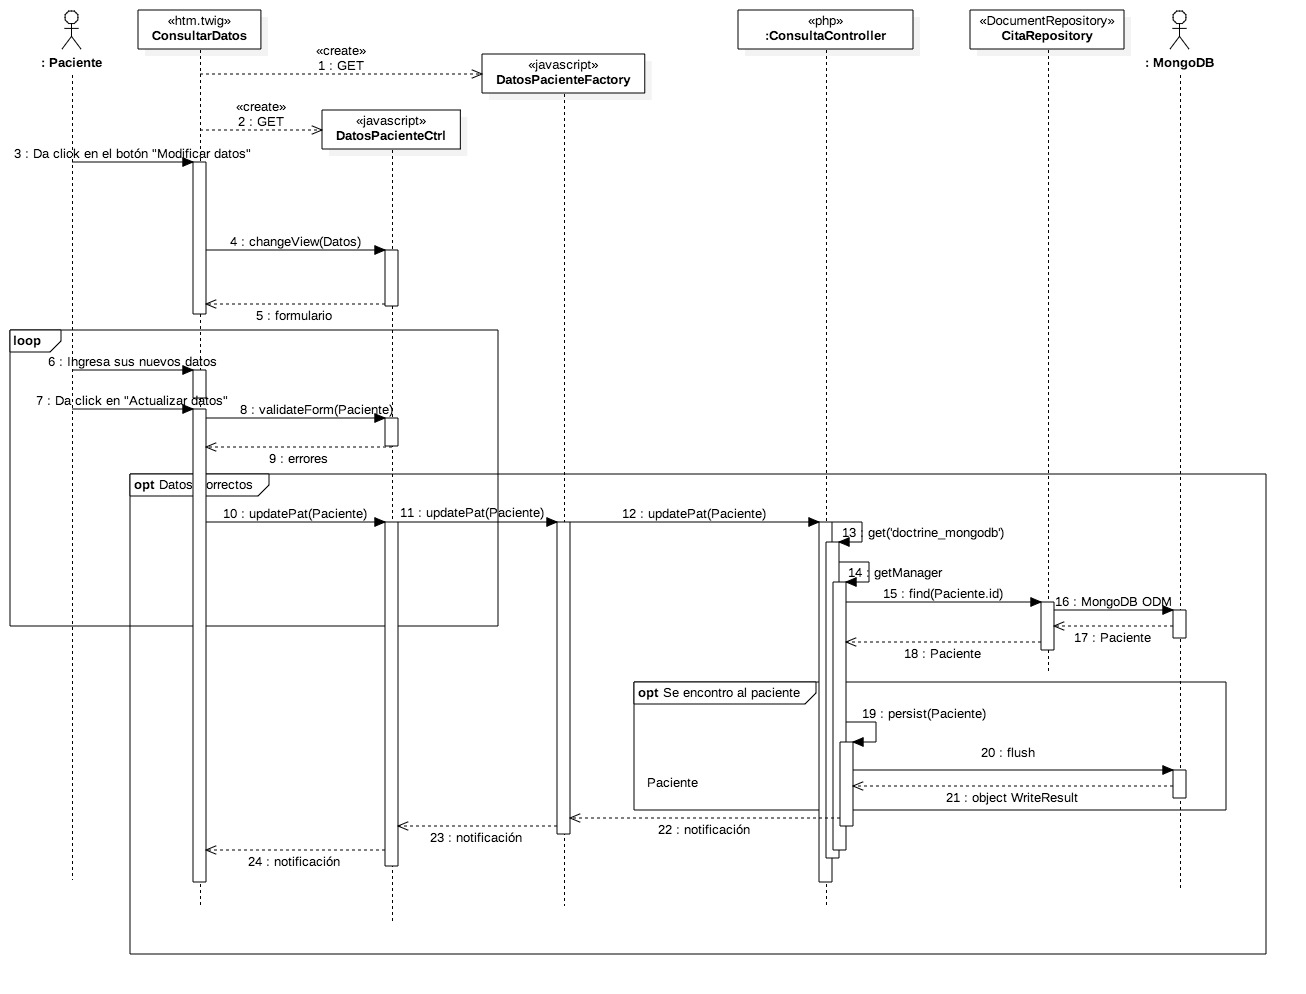
\includegraphics[width=1\textwidth]{uml/DiagramasSecuencia/AdrianGalindo/actualizarDatosPaciente}
	\caption{Actualiar datos del paciente}
\end{figure}

\newpage
\section{Agendar cita}
\begin{figure}[htbp!]
	\centering
	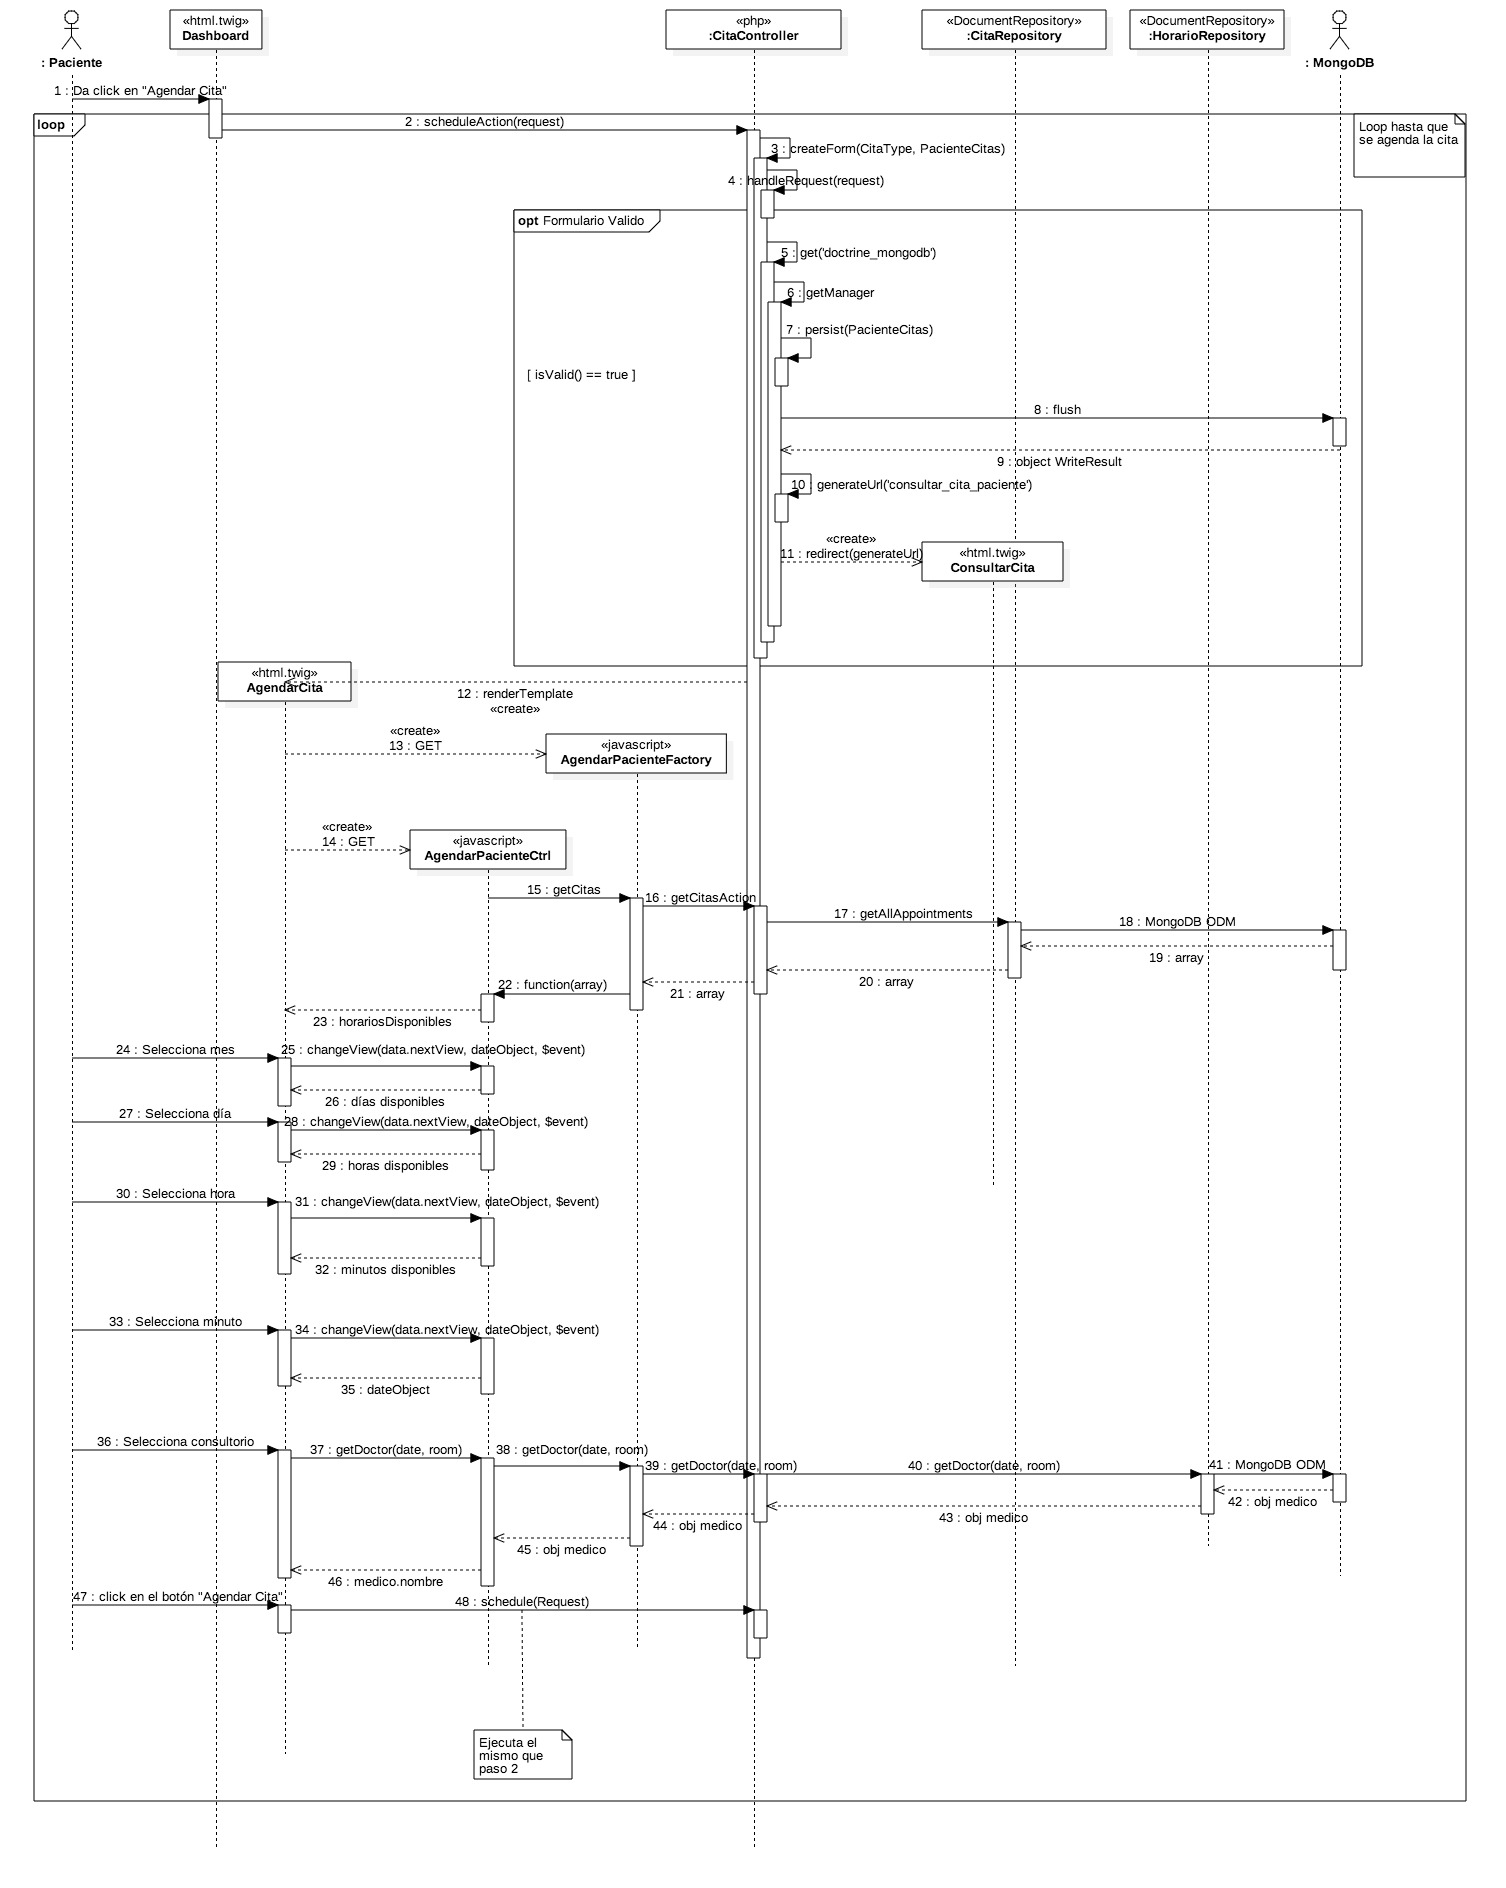
\includegraphics[width=1\textwidth]{uml/DiagramasSecuencia/AdrianGalindo/agendarCita}
	\caption{Agendar cita}
\end{figure}

\newpage

\section{Cancelar cita paciente}
\begin{figure}[htbp!]
	\centering
	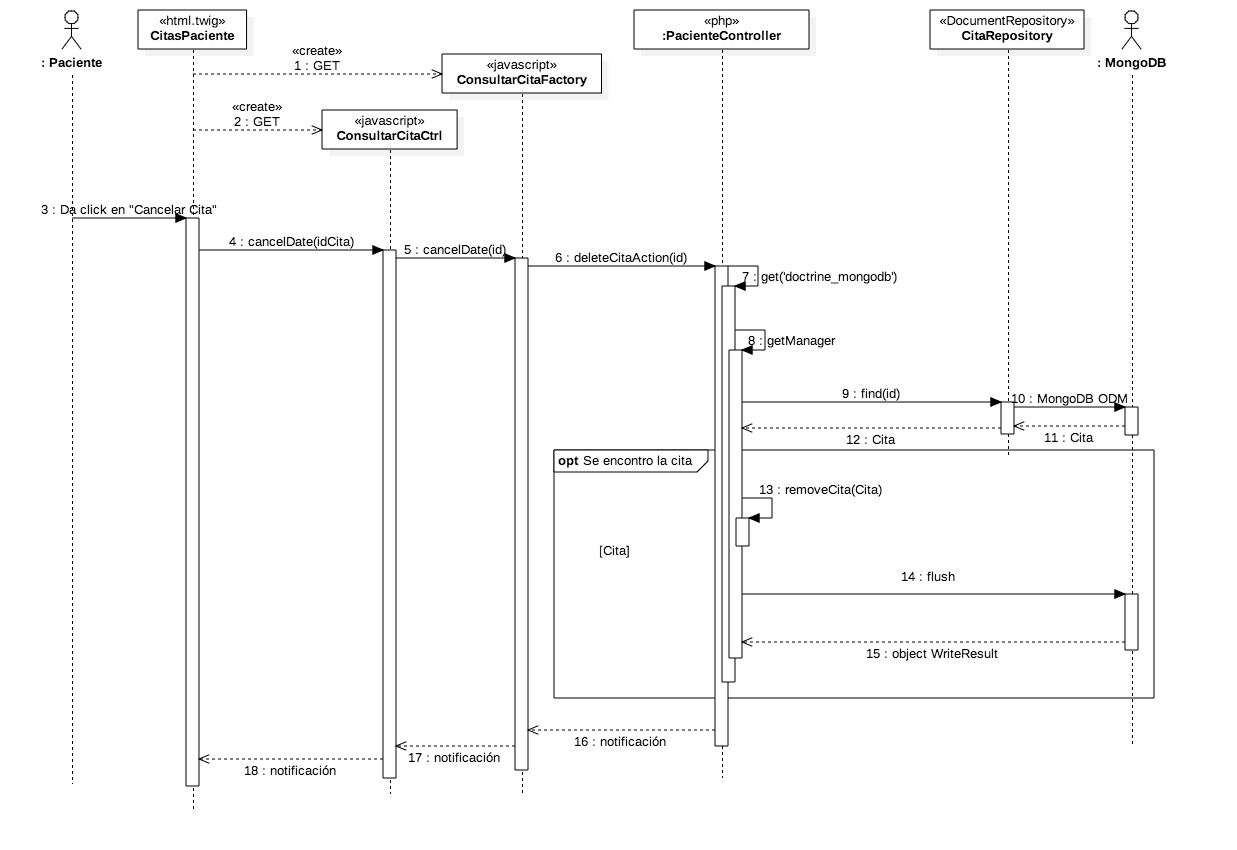
\includegraphics[width=1\textwidth]{uml/DiagramasSecuencia/AdrianGalindo/cancelarCitaPaciente}
	\caption{Cancelar cita}
\end{figure}

\newpage

\section{ Crear tratamiento}
\begin{figure}[htbp!]
	\centering
	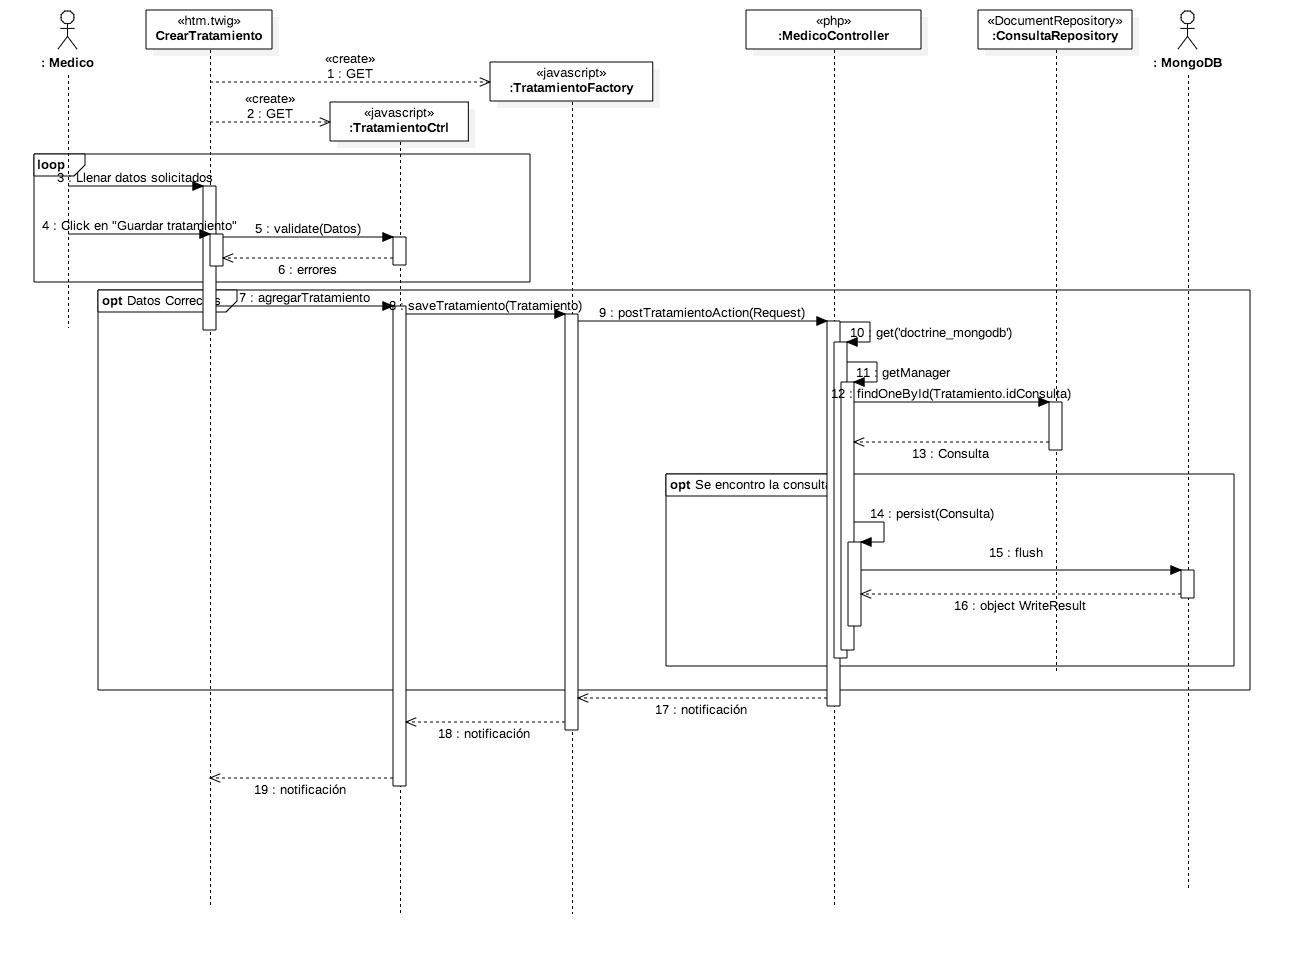
\includegraphics[width=1\textwidth]{uml/DiagramasSecuencia/AdrianGalindo/crearTratamiento}
	\caption{Crear tramatiendo}
\end{figure}

\newpage


% Pacheco

\section{Pagar cita expirada}

\begin{figure}[htbp!]
	\centering
	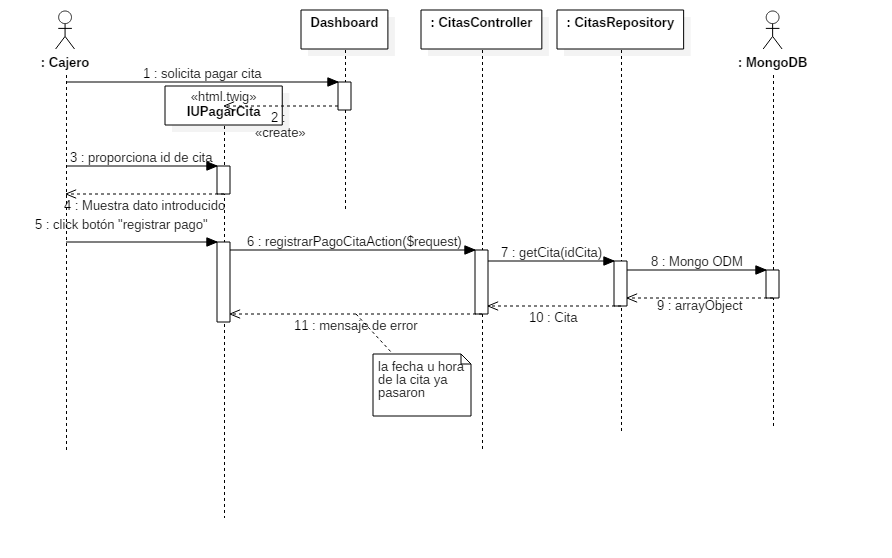
\includegraphics[width=1\textwidth]{uml/DiagramasSecuencia/DavidPacheco/pagar-cita-cita-expirada}
	\caption{Pagar cita expirada}
\end{figure}
\newpage

\section{Pagar cita inexistente}

\begin{figure}[htbp!]
	\centering
	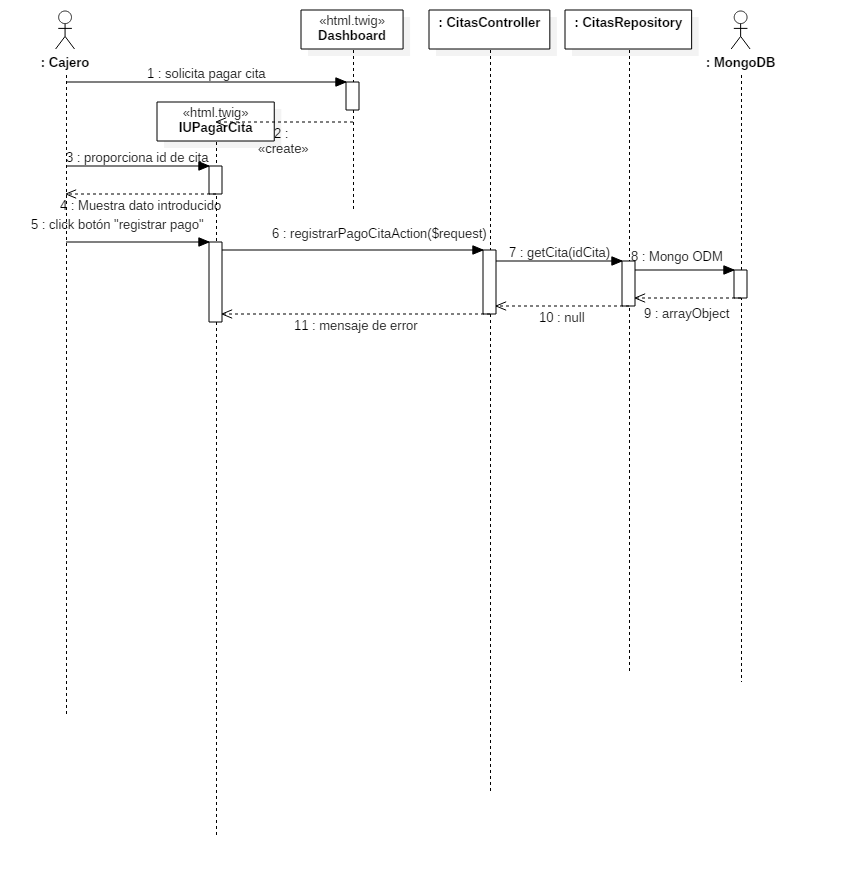
\includegraphics[width=1\textwidth]{uml/DiagramasSecuencia/DavidPacheco/pagar-cita-cita-no-existe}
	\caption{Pagar cita inexistente}
\end{figure}

\section{Pagar cita con datos incompletos}

\begin{figure}[htbp!]
	\centering
	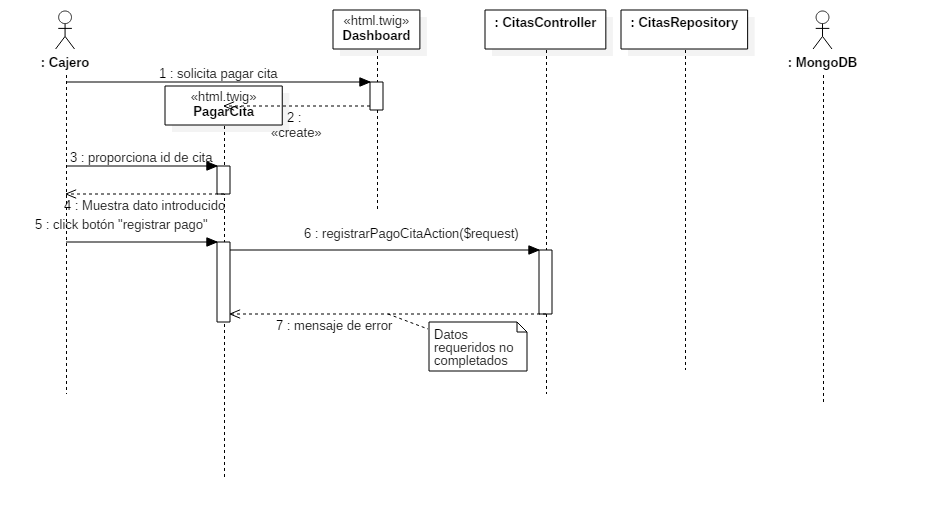
\includegraphics[width=1\textwidth]{uml/DiagramasSecuencia/DavidPacheco/pagar-cita-datos-incompletos}
	\caption{Pagar cita con datos incompletos}
\end{figure}

\section{Pagar cita con datos incorrectos}

\begin{figure}[htbp!]
	\centering
	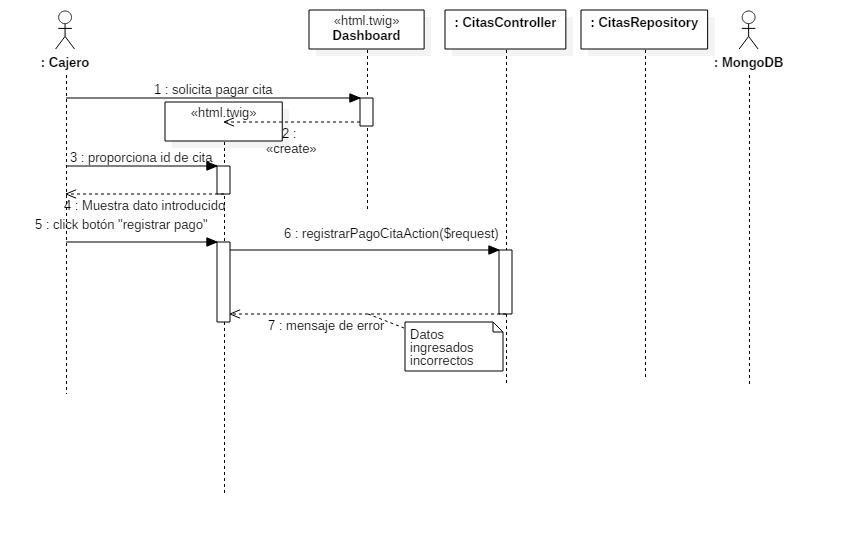
\includegraphics[width=1\textwidth]{uml/DiagramasSecuencia/DavidPacheco/pagar-cita-datos-incorrectos}
	\caption{Pagar cita con datos incorrectos}
\end{figure}

\section{ Pagar cita}

\begin{figure}[htbp!]
	\centering
	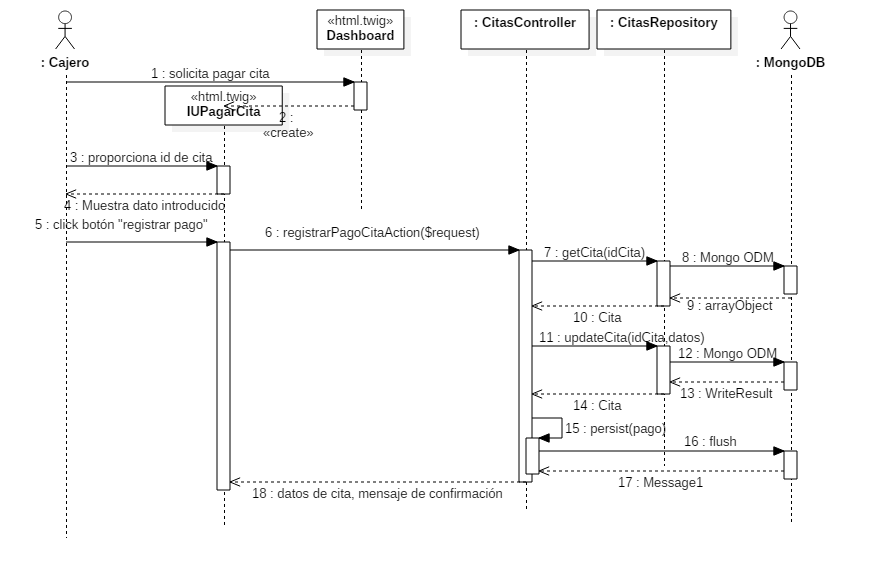
\includegraphics[width=1\textwidth]{uml/DiagramasSecuencia/DavidPacheco/pagar-cita}
	\caption{Pagar cita}
\end{figure}

\section{ Registrar Expediente}

\begin{figure}[htbp!]
	\centering
	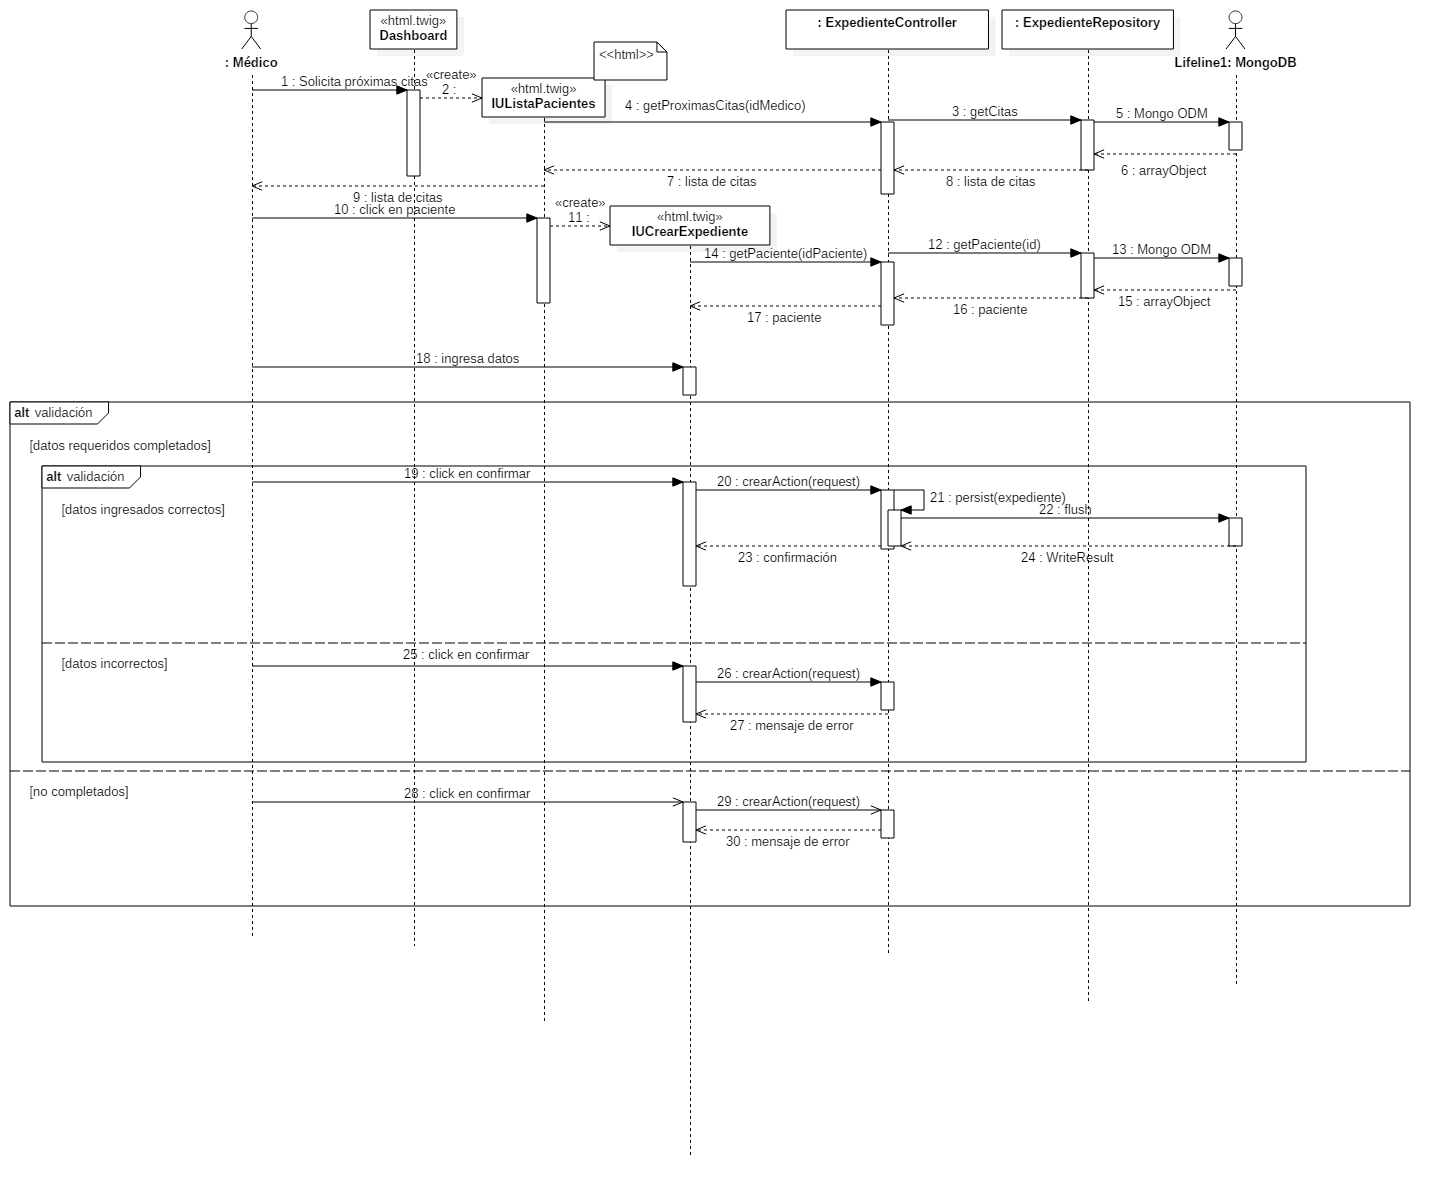
\includegraphics[width=1\textwidth]{uml/DiagramasSecuencia/DavidPacheco/registrar-expediente}
	\caption{Registrar Expediente}
\end{figure}

\section{ Registrar médico con correo ya existente}

\begin{figure}[htbp!]
	\centering
	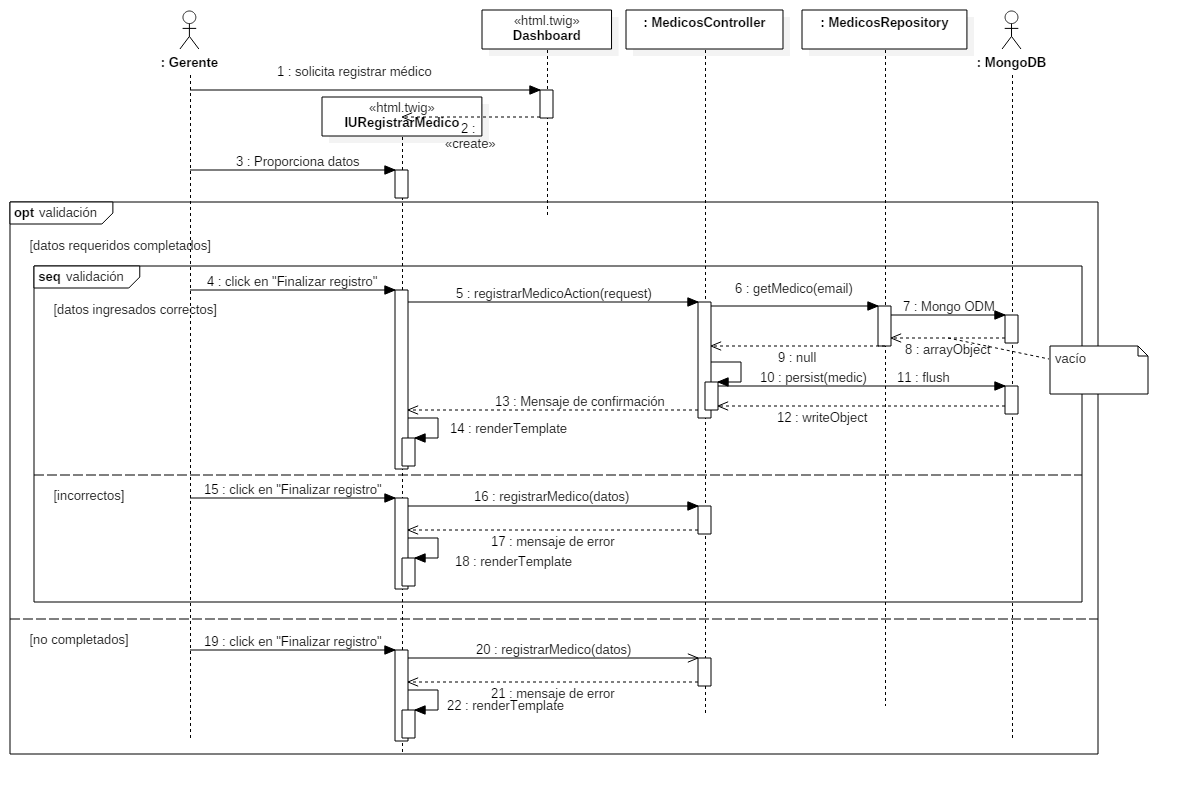
\includegraphics[width=1\textwidth]{uml/DiagramasSecuencia/DavidPacheco/registrar-medico}
	\caption{Registrar médico con correo ya existente}
\end{figure}

\section{Registrar médico}

\begin{figure}[htbp!]
	\centering
	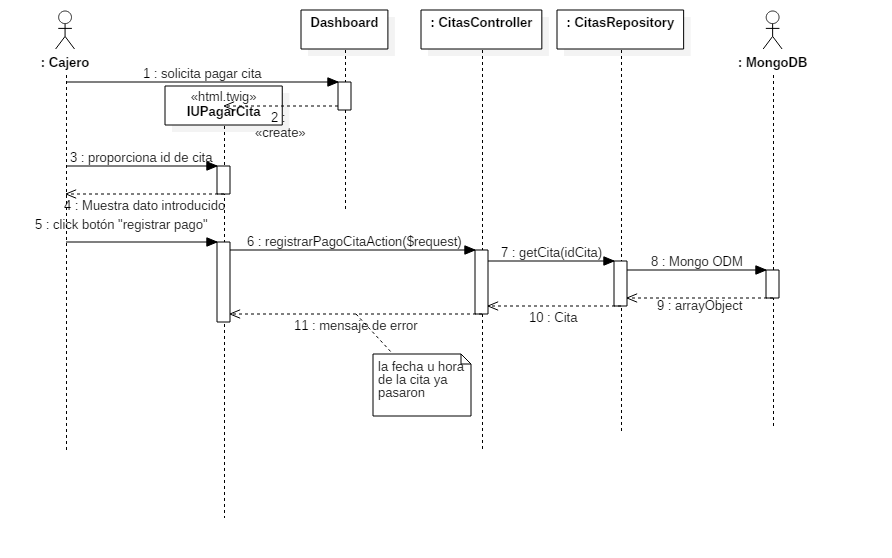
\includegraphics[width=1\textwidth]{uml/DiagramasSecuencia/DavidPacheco/pagar-cita-cita-expirada}
	\caption{Registrar médico}
\end{figure}

\section{Registrar paciente ya existente (actor paciente)}

\section{Registrar paciente (actor paciente)}

%Demis

\section{Consultar citas paciente}
	\begin{figure}[htbp!]
		\centering
			\includegraphics[width=1\textwidth]{uml/DiagramasSecuencia/DemisGomez/consultarCitasPaciente}
		\caption{Consultas citas paciente}
	\end{figure}
	\newpage
\section{Consultar inventario}
	\begin{figure}[htbp!]
		\centering
			\includegraphics[width=1\textwidth]{uml/DiagramasSecuencia/DemisGomez/consultarInventario}
		\caption{Consultas inventario}
	\end{figure}
	\newpage
\section{Consultar pacientes}
	\begin{figure}[htbp!]
		\centering
			\includegraphics[width=1\textwidth]{uml/DiagramasSecuencia/DemisGomez/consultarPacientes}
		\caption{Consultas pacientes}
	\end{figure}
	\newpage
\section{Modificar Inventario}
	\begin{figure}[htbp!]
		\centering
			\includegraphics[width=1\textwidth]{uml/DiagramasSecuencia/DemisGomez/modificarInventario}
		\caption{Modificar inventario}
	\end{figure}
	\newpage

%Trujillo
\newpage
\section{Consultar citas enfermera}
\begin{figure}[htbp!]
		\centering
			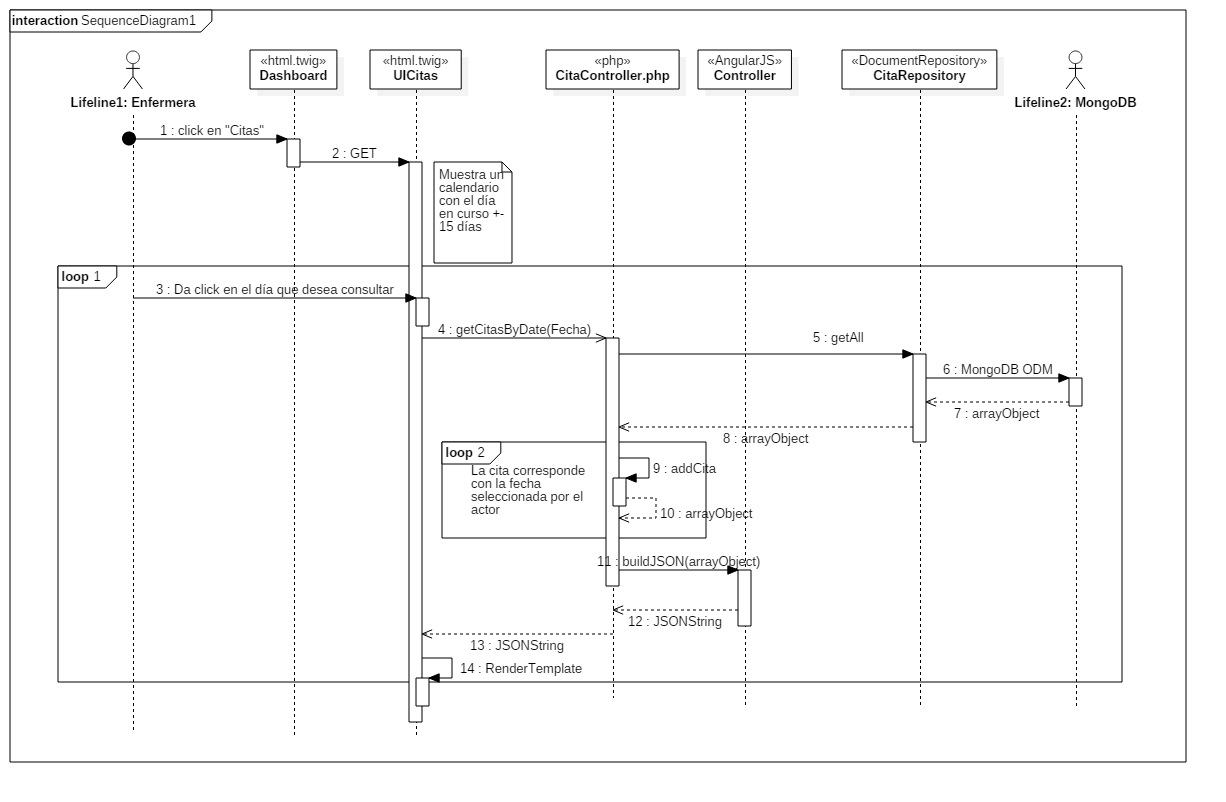
\includegraphics[width=1\textwidth]{uml/DiagramasSecuencia/Trujillo/getCitasEnfermera}
		\caption{Consultas citas enfermera}
	\end{figure}
	\newpage
\section{Consultar datos paciente}
\begin{figure}[htbp!]
		\centering
			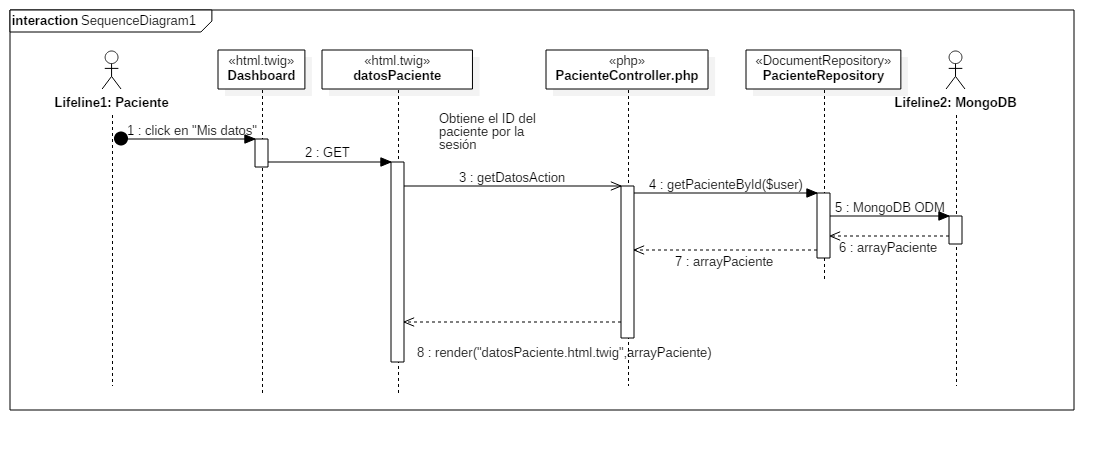
\includegraphics[width=1\textwidth]{uml/DiagramasSecuencia/Trujillo/getDatosPaciente}
		\caption{Consultar datos paciente}
	\end{figure}
	\newpage
\section{Registrar pago farmacia}
\begin{figure}[htbp!]
		\centering
			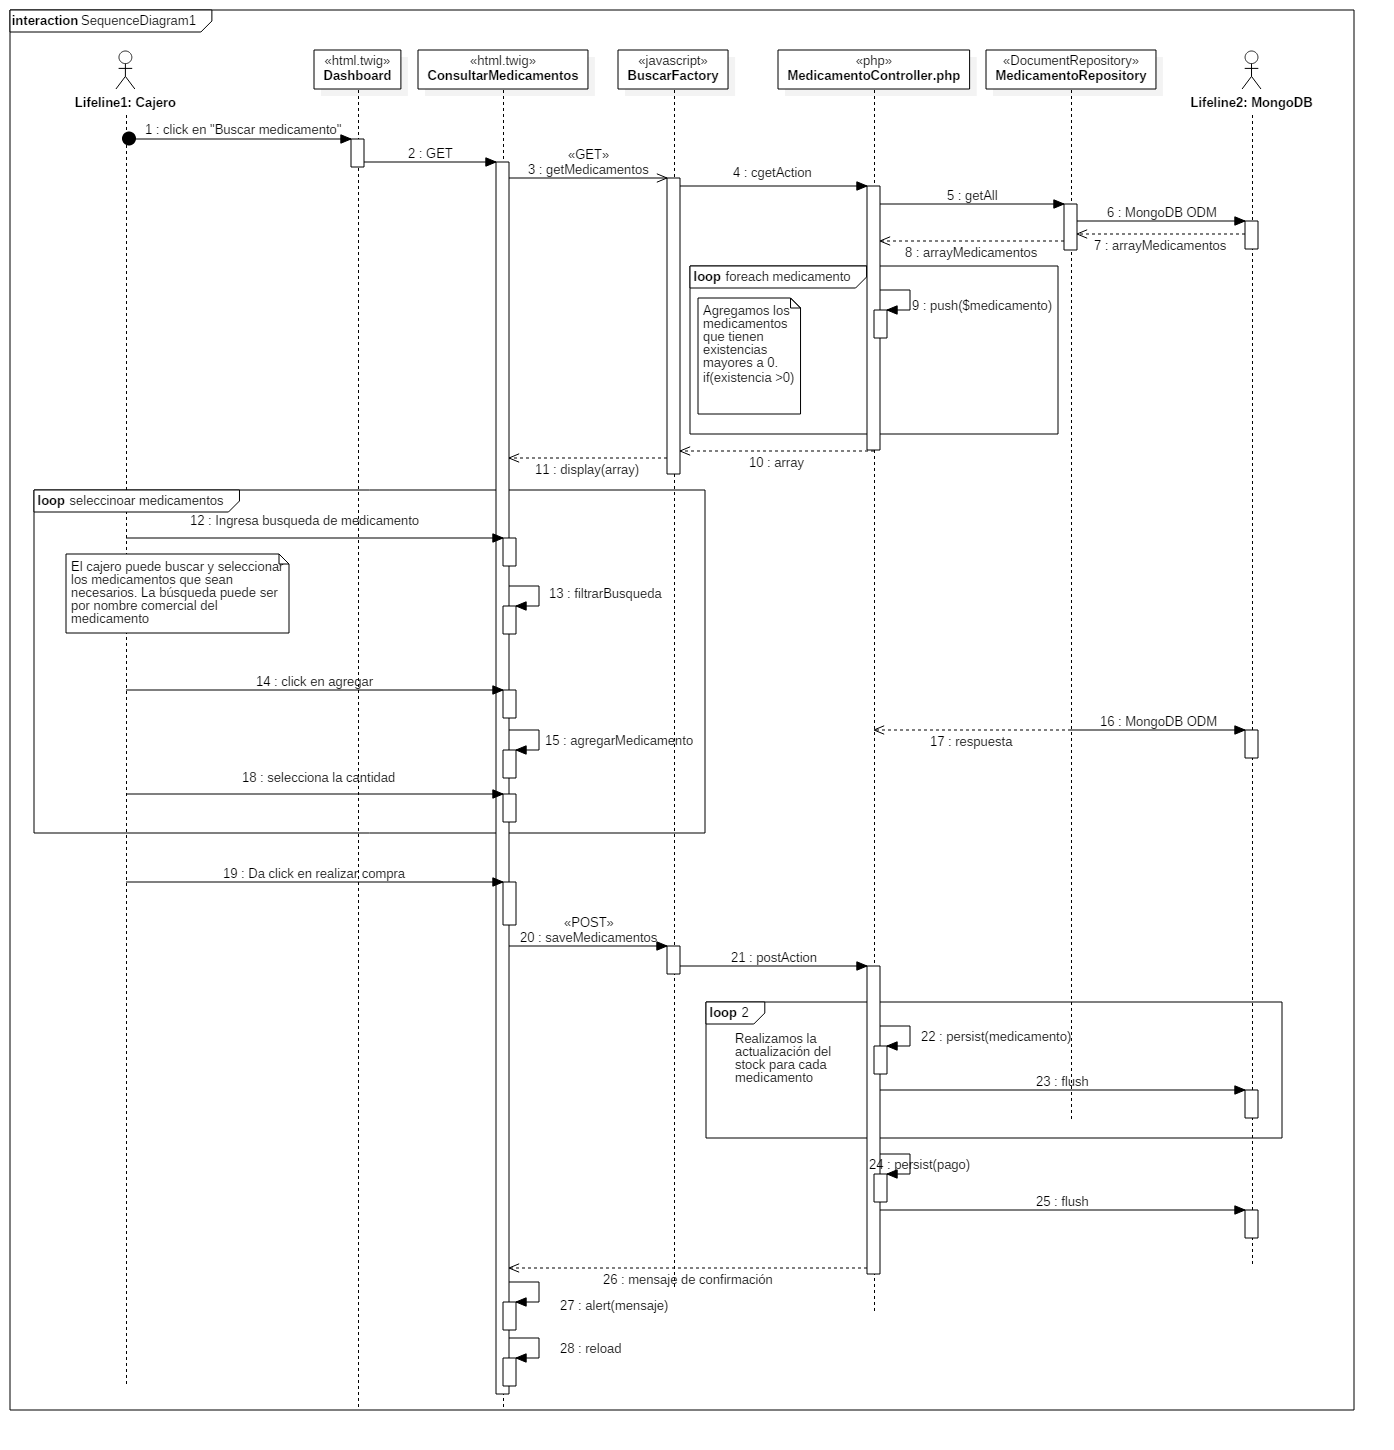
\includegraphics[width=1\textwidth]{uml/DiagramasSecuencia/Trujillo/insertPagoMedicina}
		\caption{Insertar pago farmacia}
	\end{figure}
	\newpage
\section{Modificar horario médico}
\begin{figure}[htbp!]
		\centering
			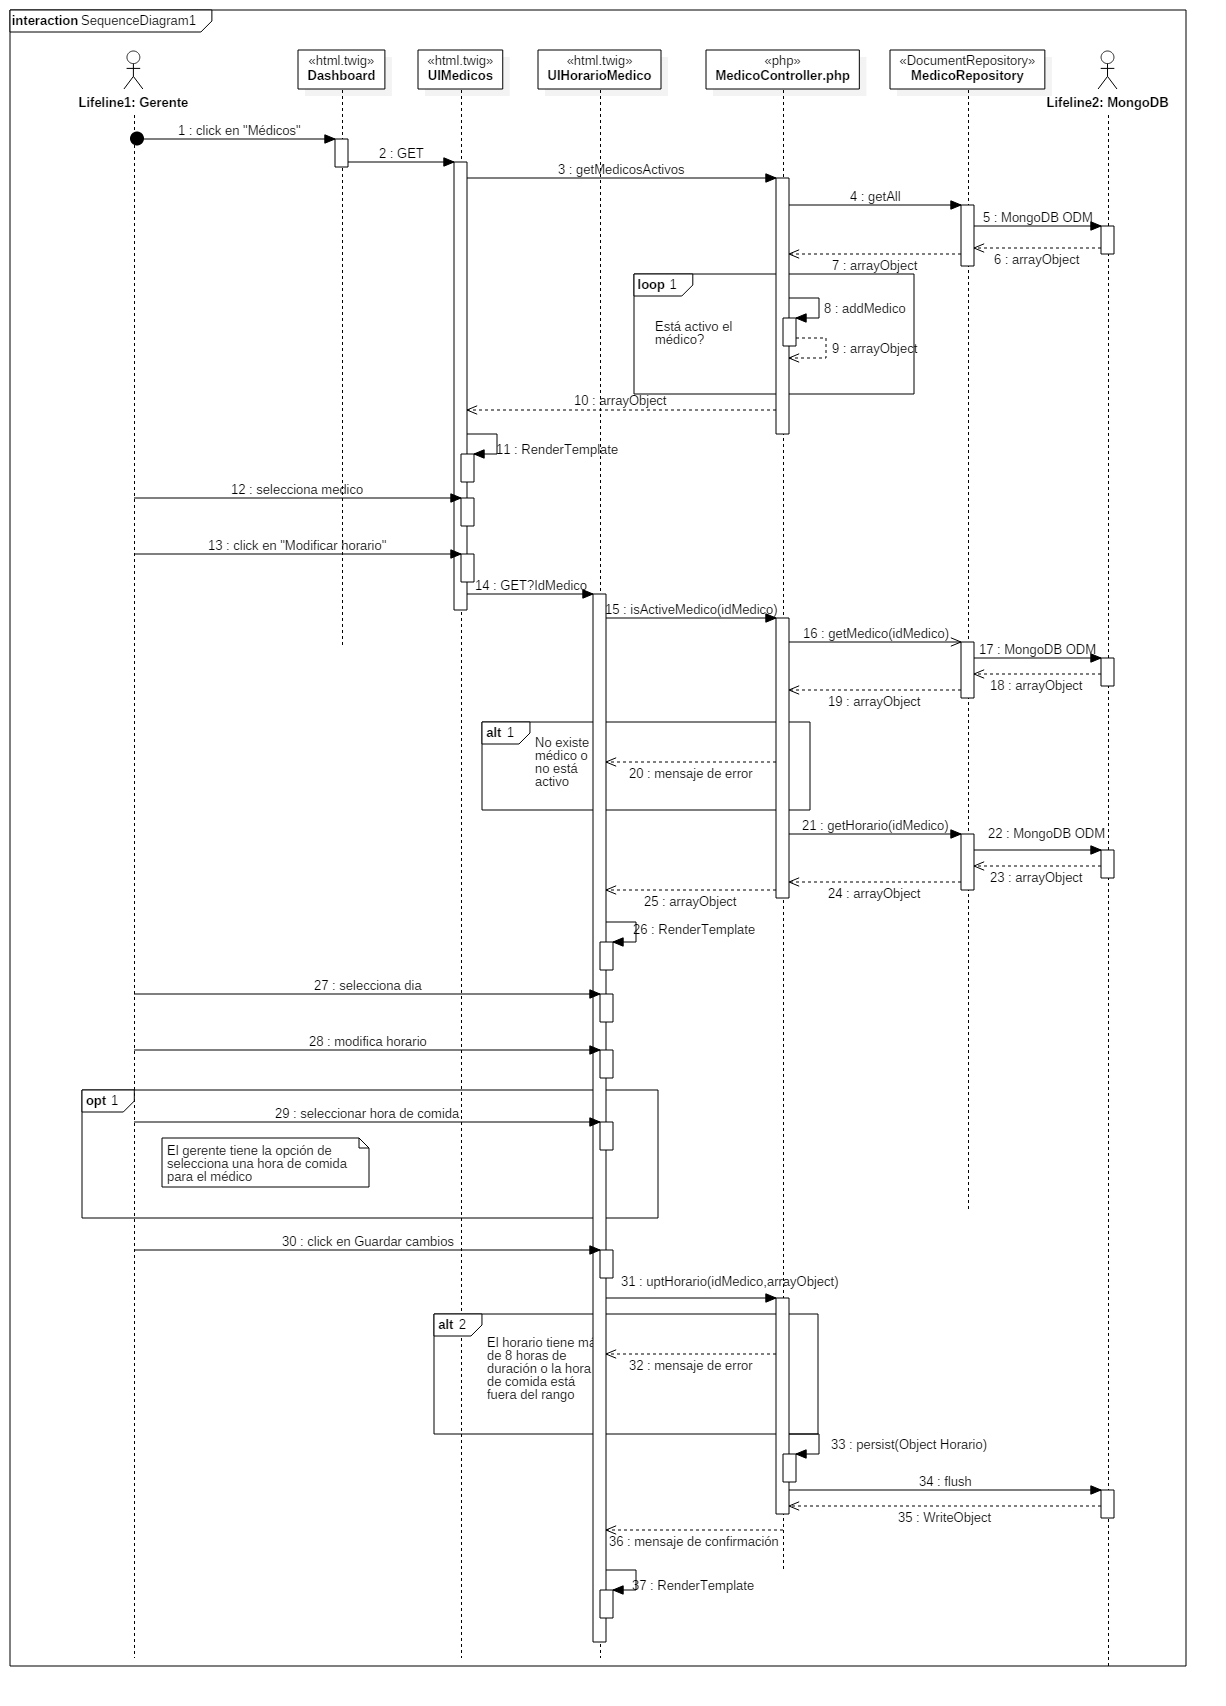
\includegraphics[width=0.8\textwidth]{uml/DiagramasSecuencia/Trujillo/uptHorario}
		\caption{Modificar horario médico}
	\end{figure}
	\newpage

%Ruben
\newpage
\section{Consultas diarias (actor gerente)}
\begin{figure}[htbp!]
		\centering
			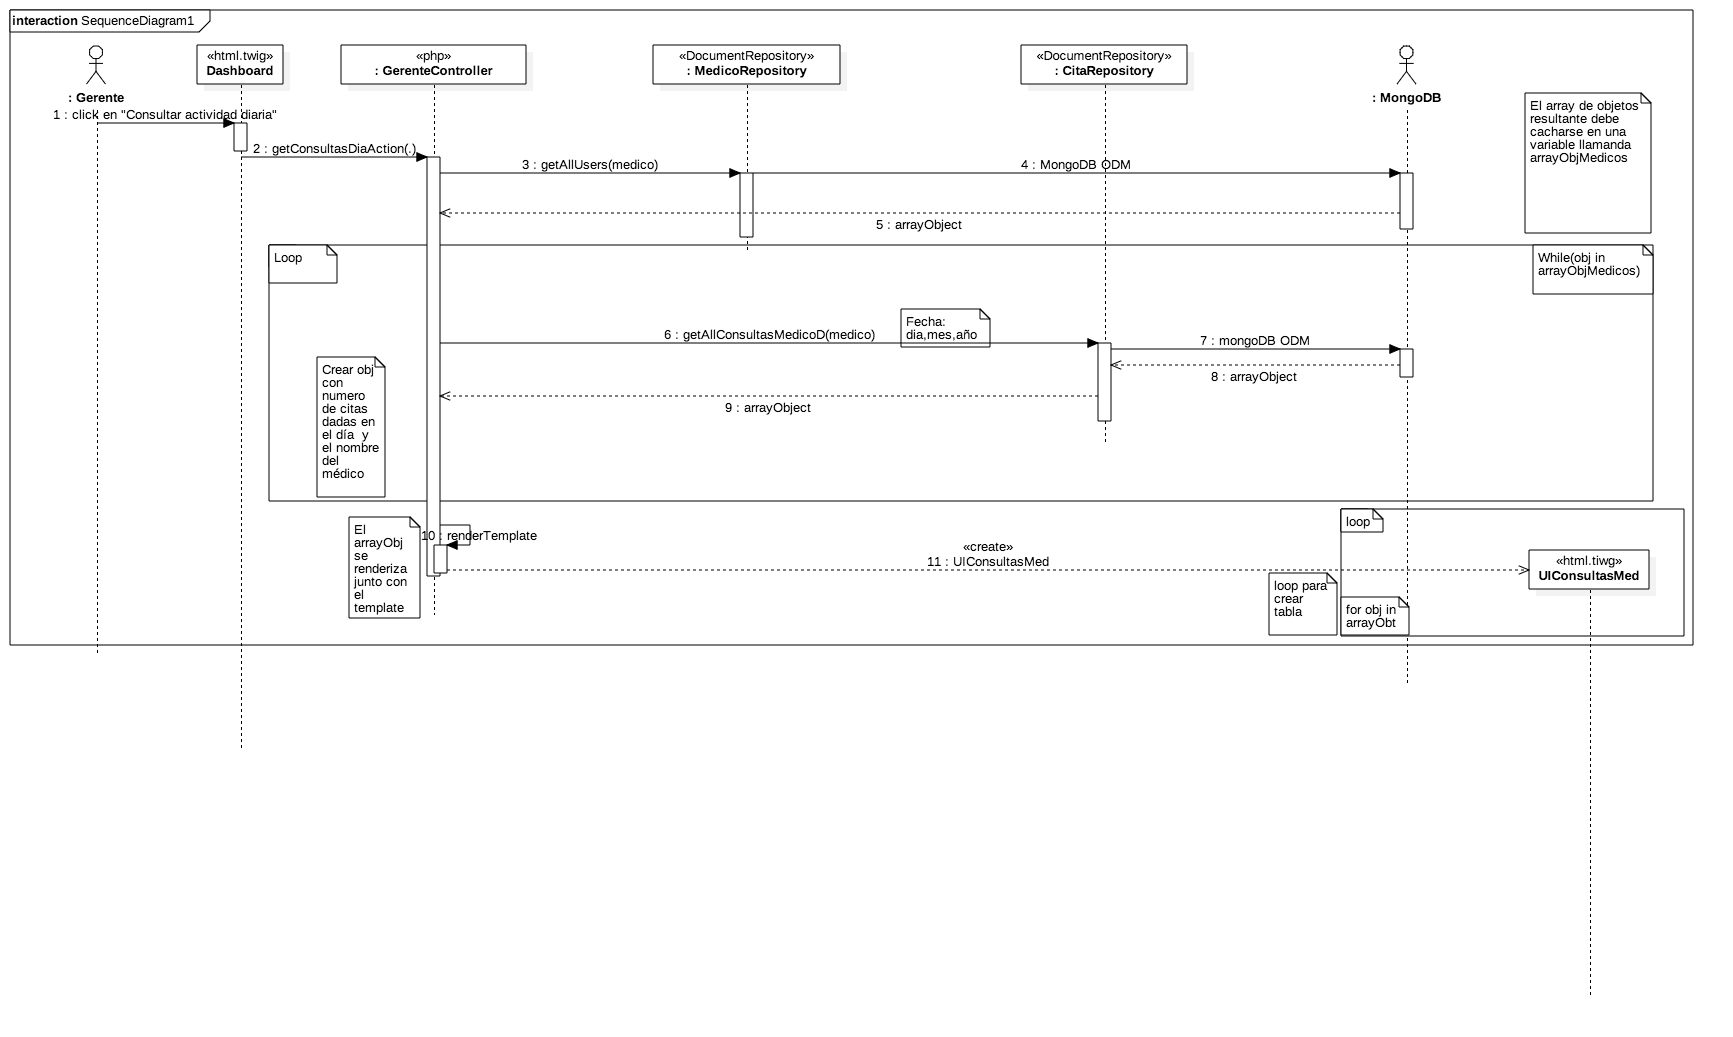
\includegraphics[width=1\textwidth]{uml/DiagramasSecuencia/RubenMurga/getConsultasDia}
		\caption{Consultas diarias}
	\end{figure}

\newpage
\section{Consultas mensuales (actor gerente)}

\begin{figure}[htbp!]
		\centering
			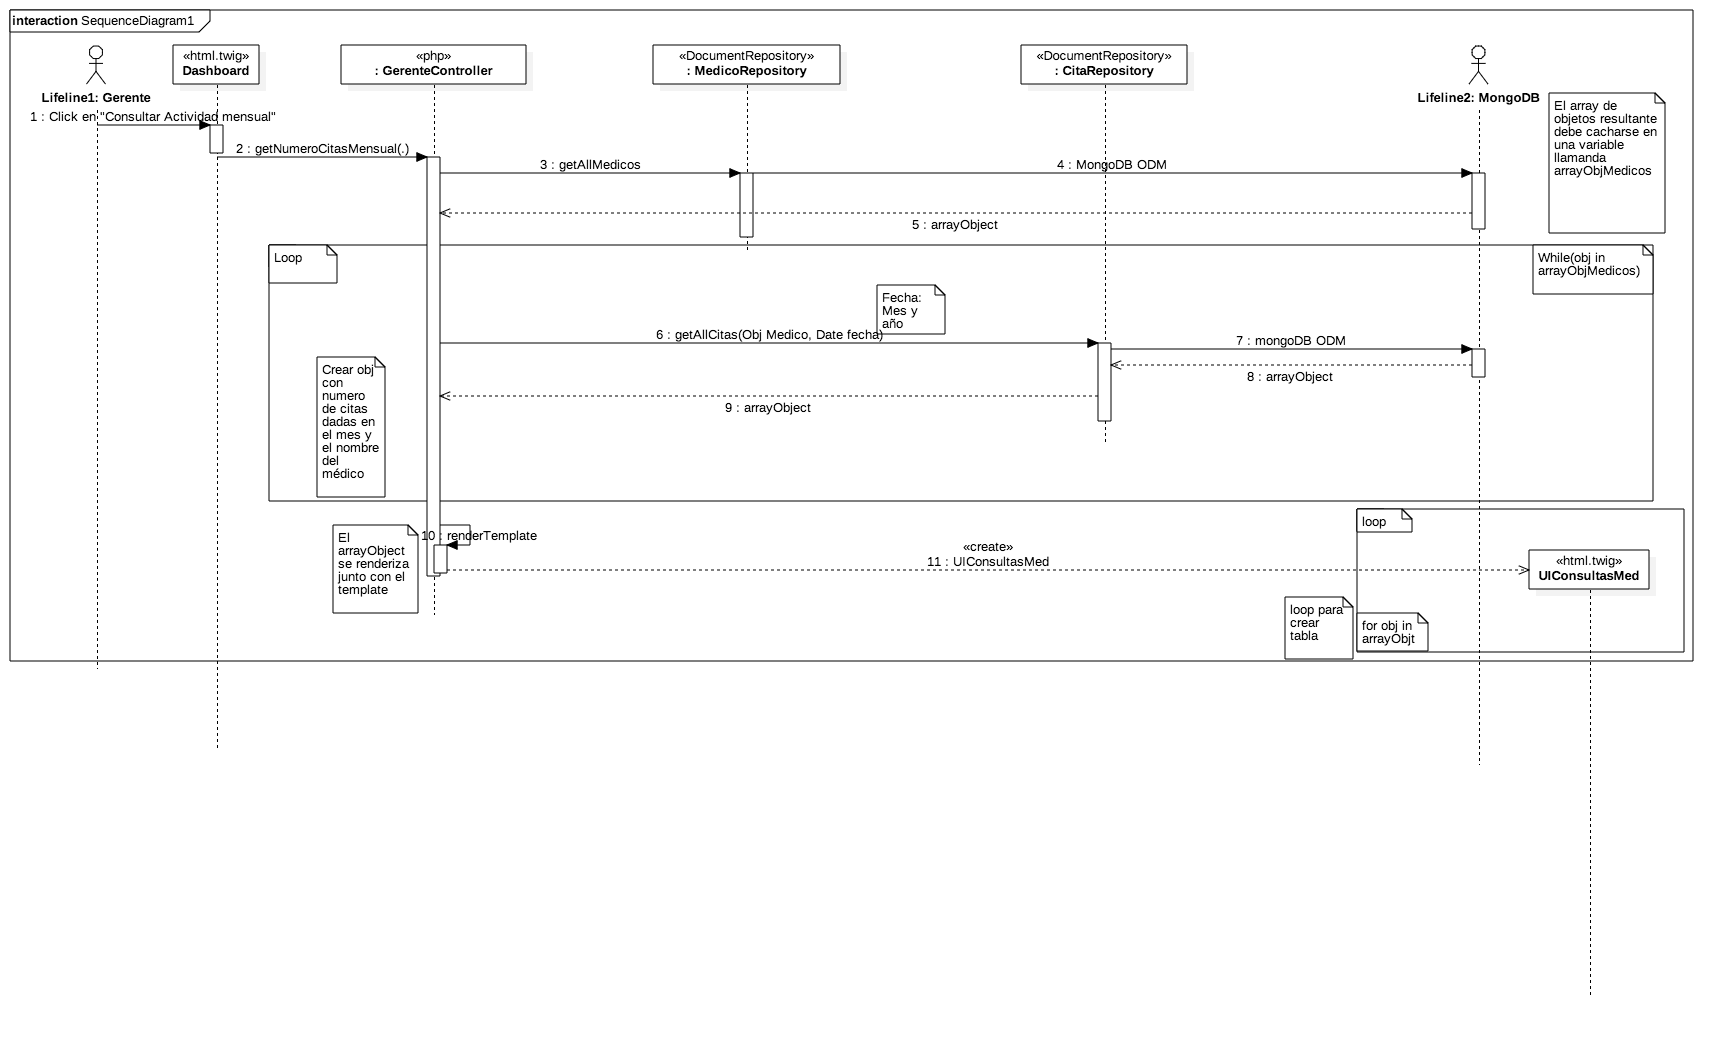
\includegraphics[width=1\textwidth]{uml/DiagramasSecuencia/RubenMurga/getConsultasMes}
		\caption{Consultas mensuales}
	\end{figure}

\newpage
\section{Consultar expediente}
\begin{figure}[htbp!]
		\centering
			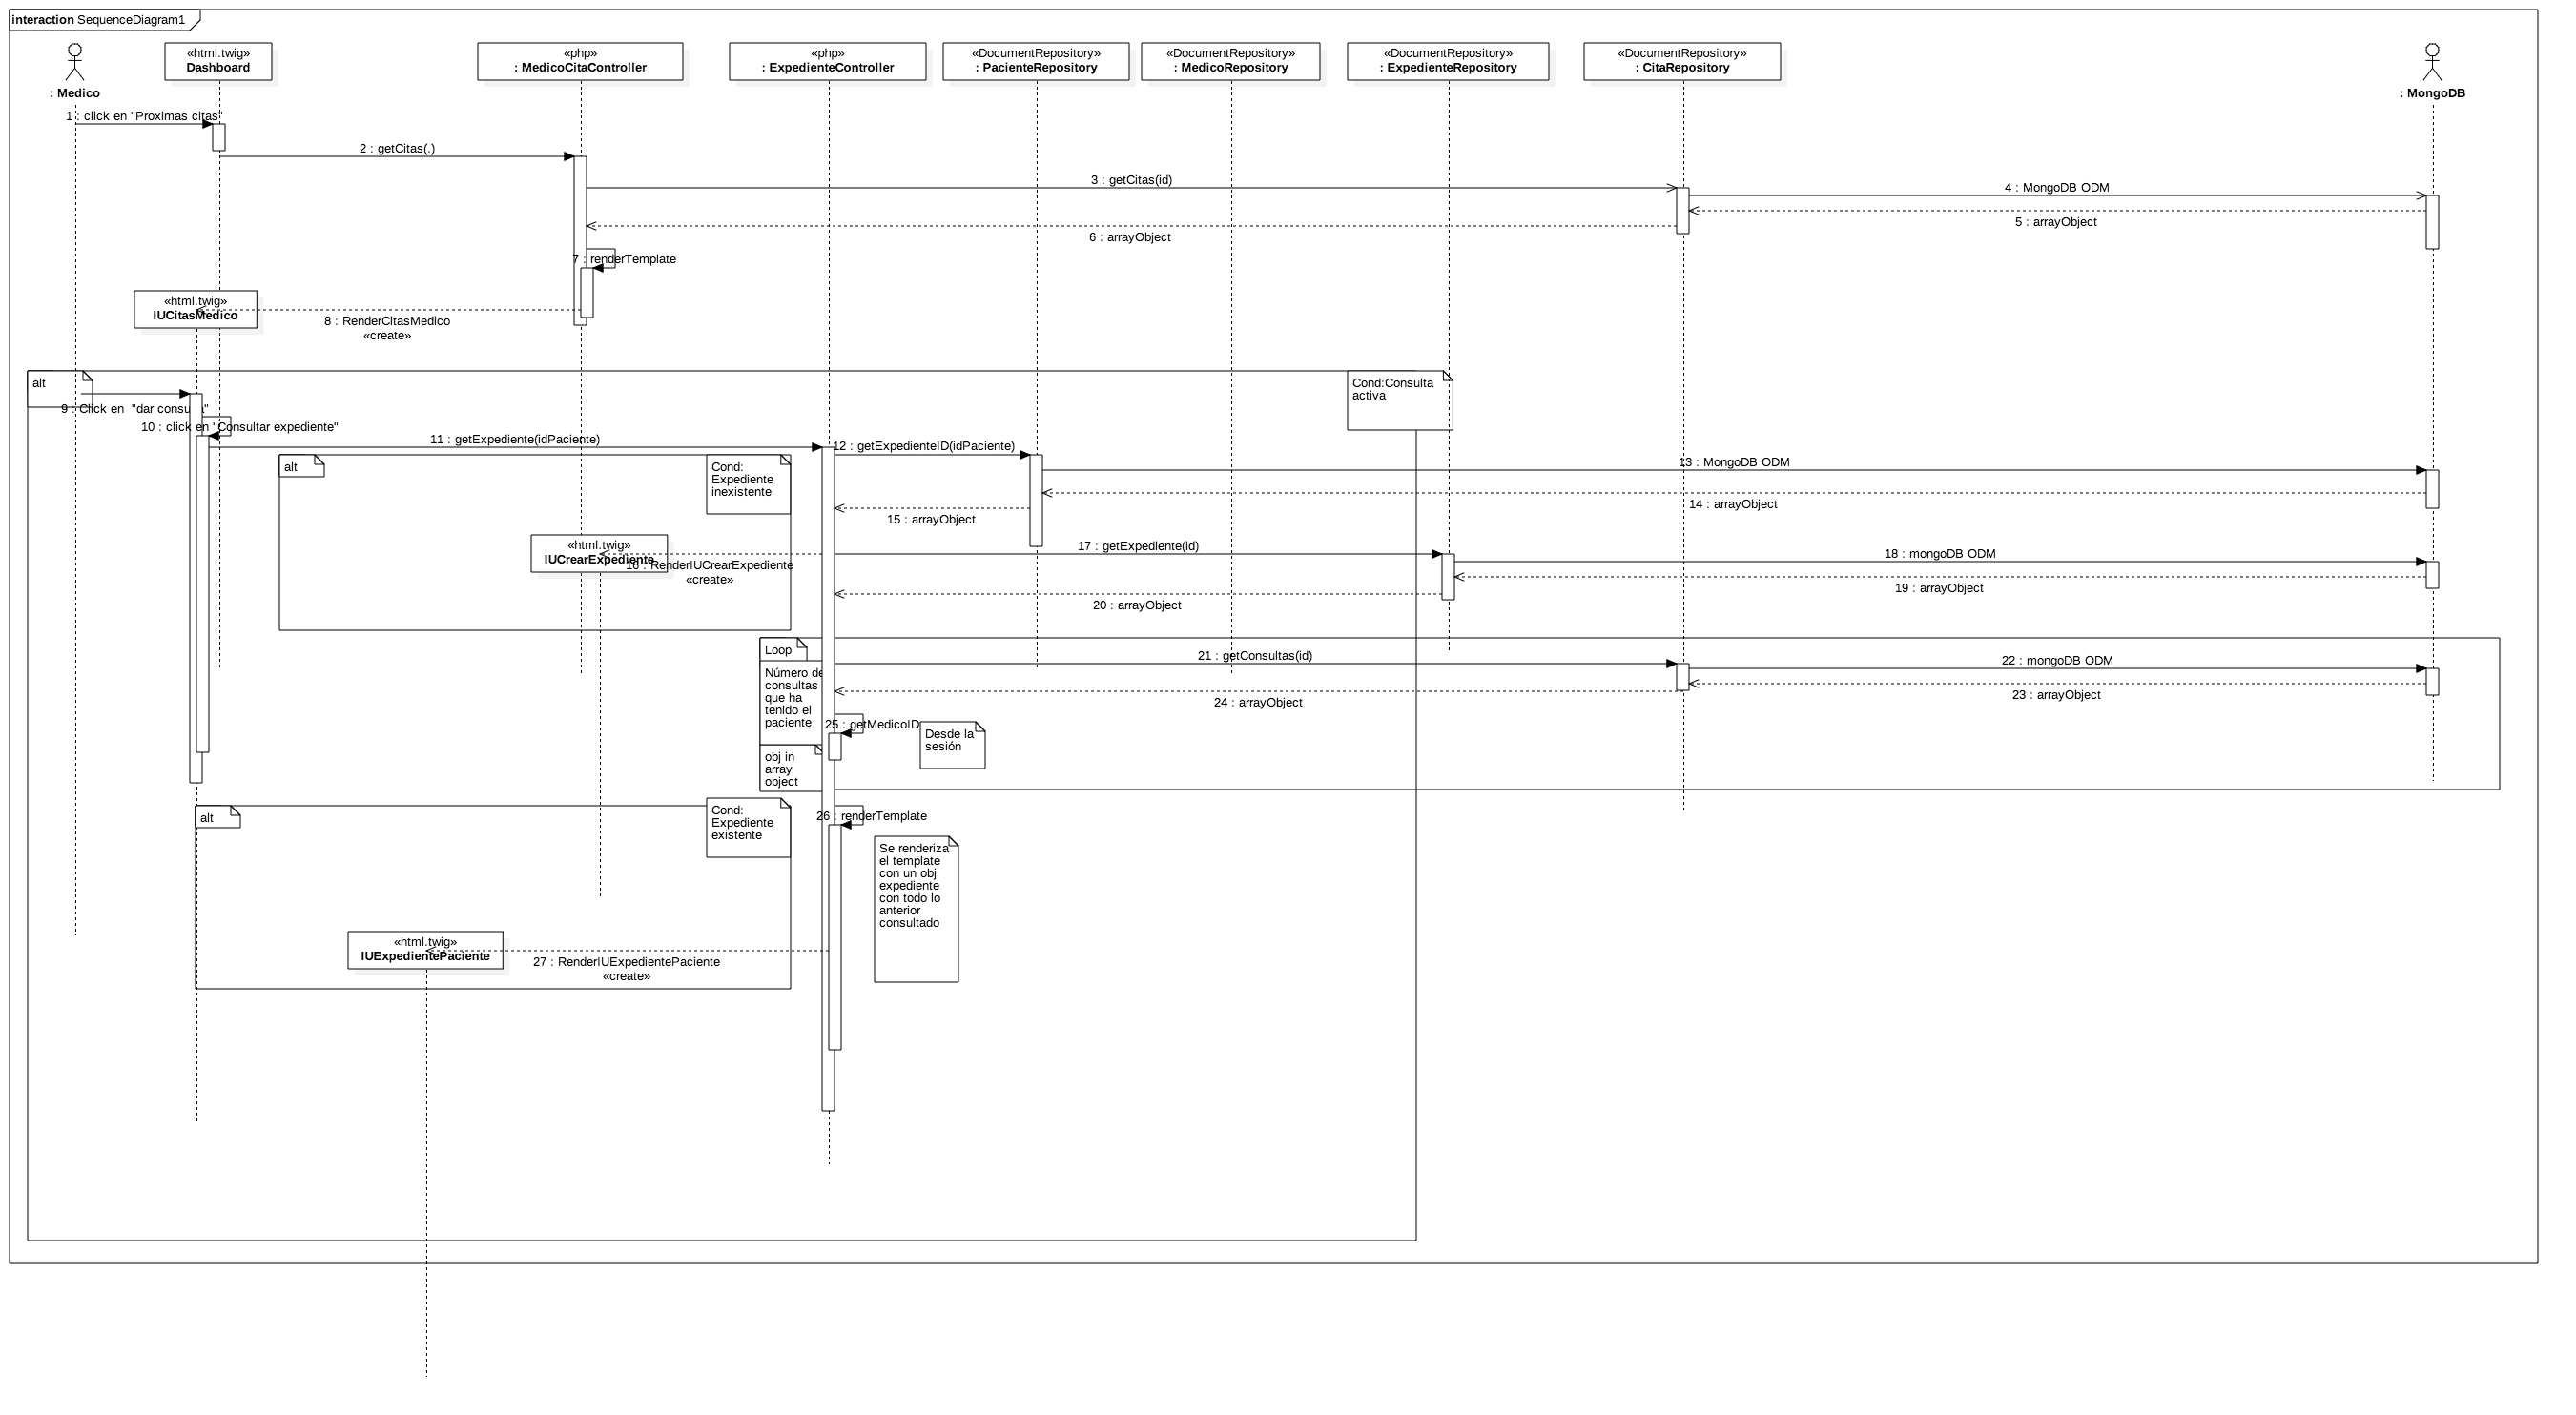
\includegraphics[width=1\textwidth]{uml/DiagramasSecuencia/RubenMurga/getExpediente}
		\caption{Consultar Expediente}
	\end{figure}
\newpage
\section{Consultar ventas diarias (actor gerente)}
\begin{figure}[htbp!]
		\centering
			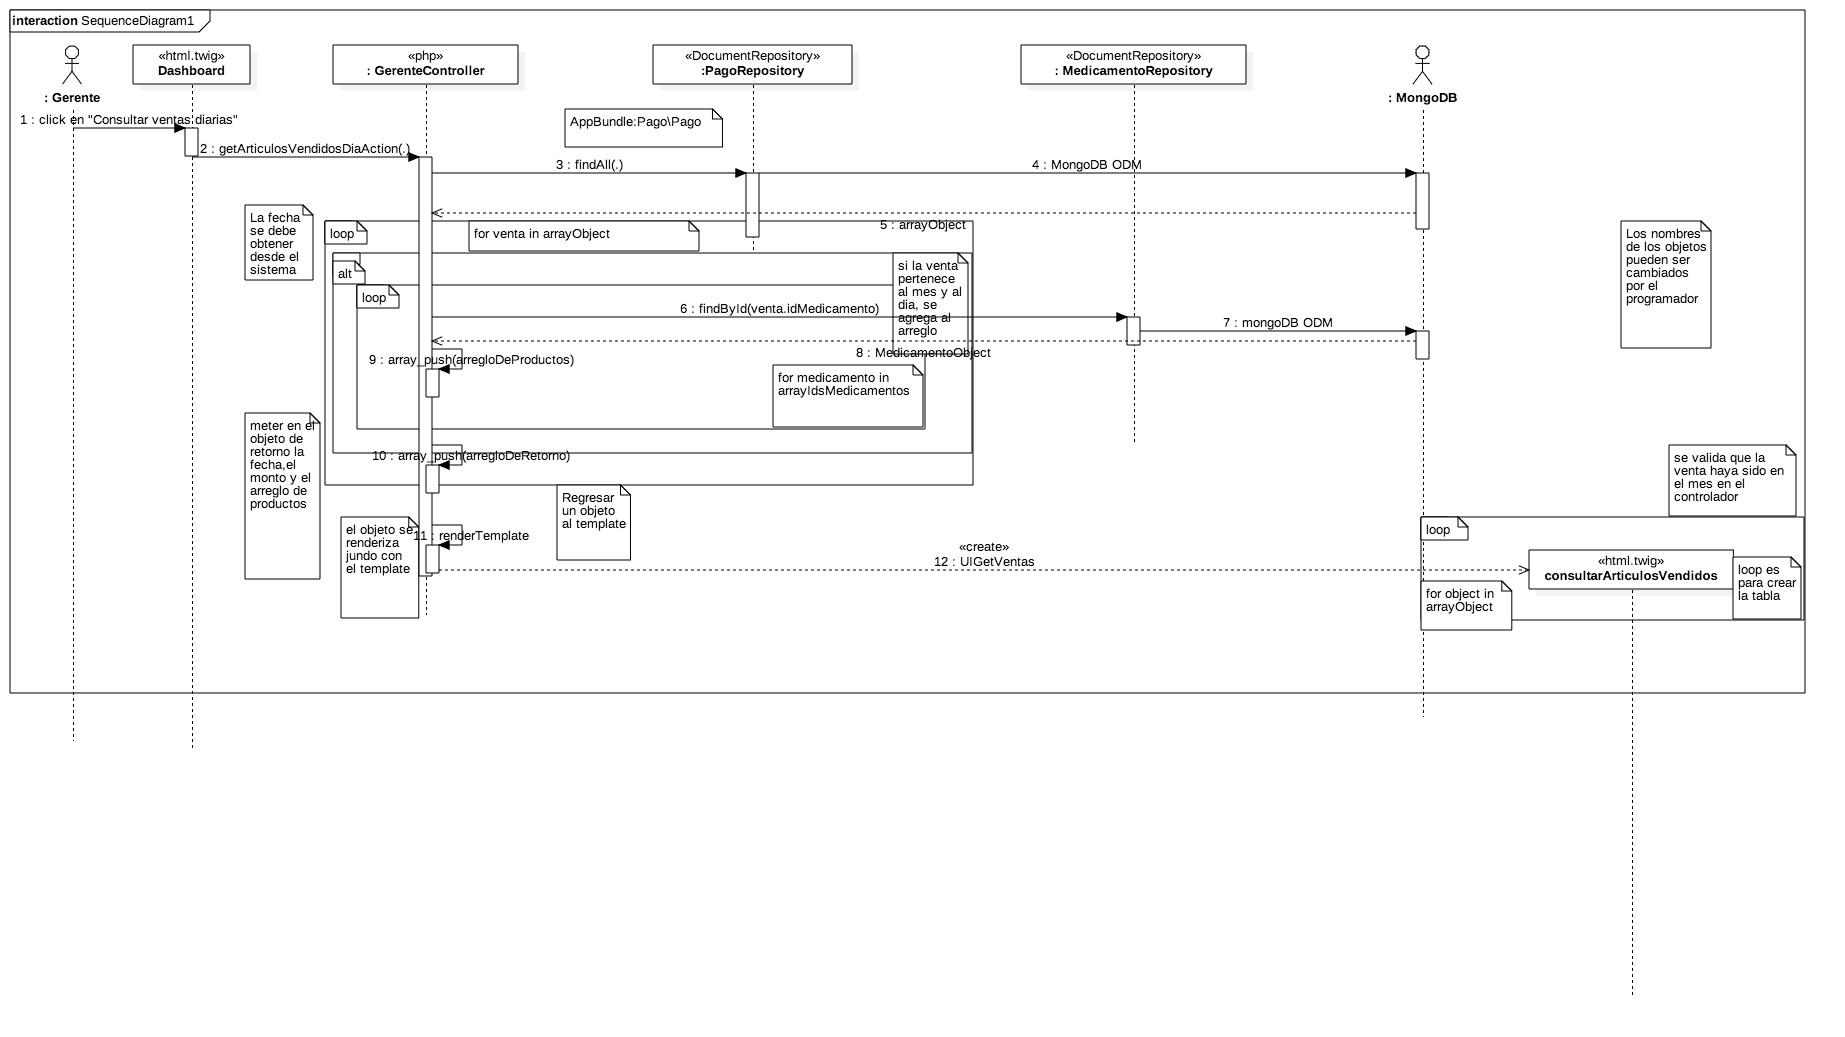
\includegraphics[width=1\textwidth]{uml/DiagramasSecuencia/RubenMurga/getVentasDia}
		\caption{Cosultar ventas diarias}
	\end{figure}
\newpage
\section{Consultar ventas mes (actor gerente)}
\begin{figure}[htbp!]
		\centering
			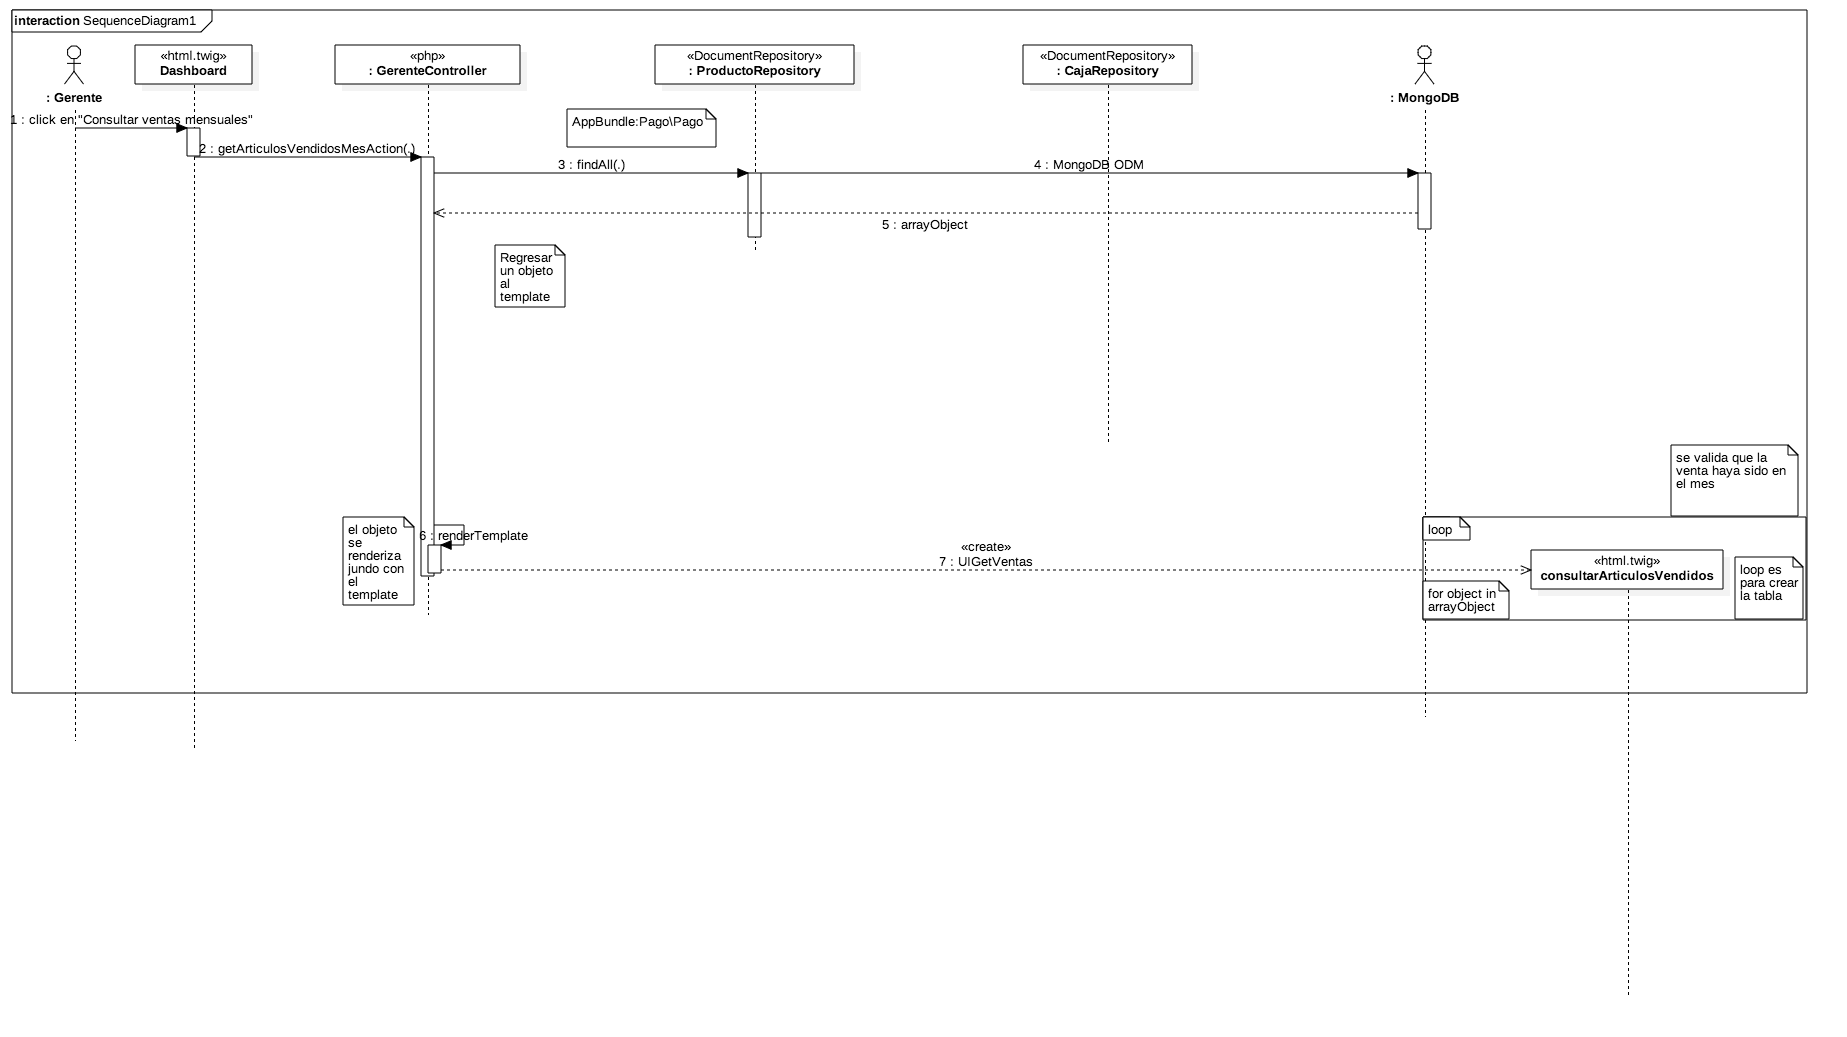
\includegraphics[width=1\textwidth]{uml/DiagramasSecuencia/RubenMurga/getVentasMes}
		\caption{Consultar ventas mensuales}
	\end{figure}
\newpage
\section{Registrar paciente}
\begin{figure}[htbp!]
		\centering
			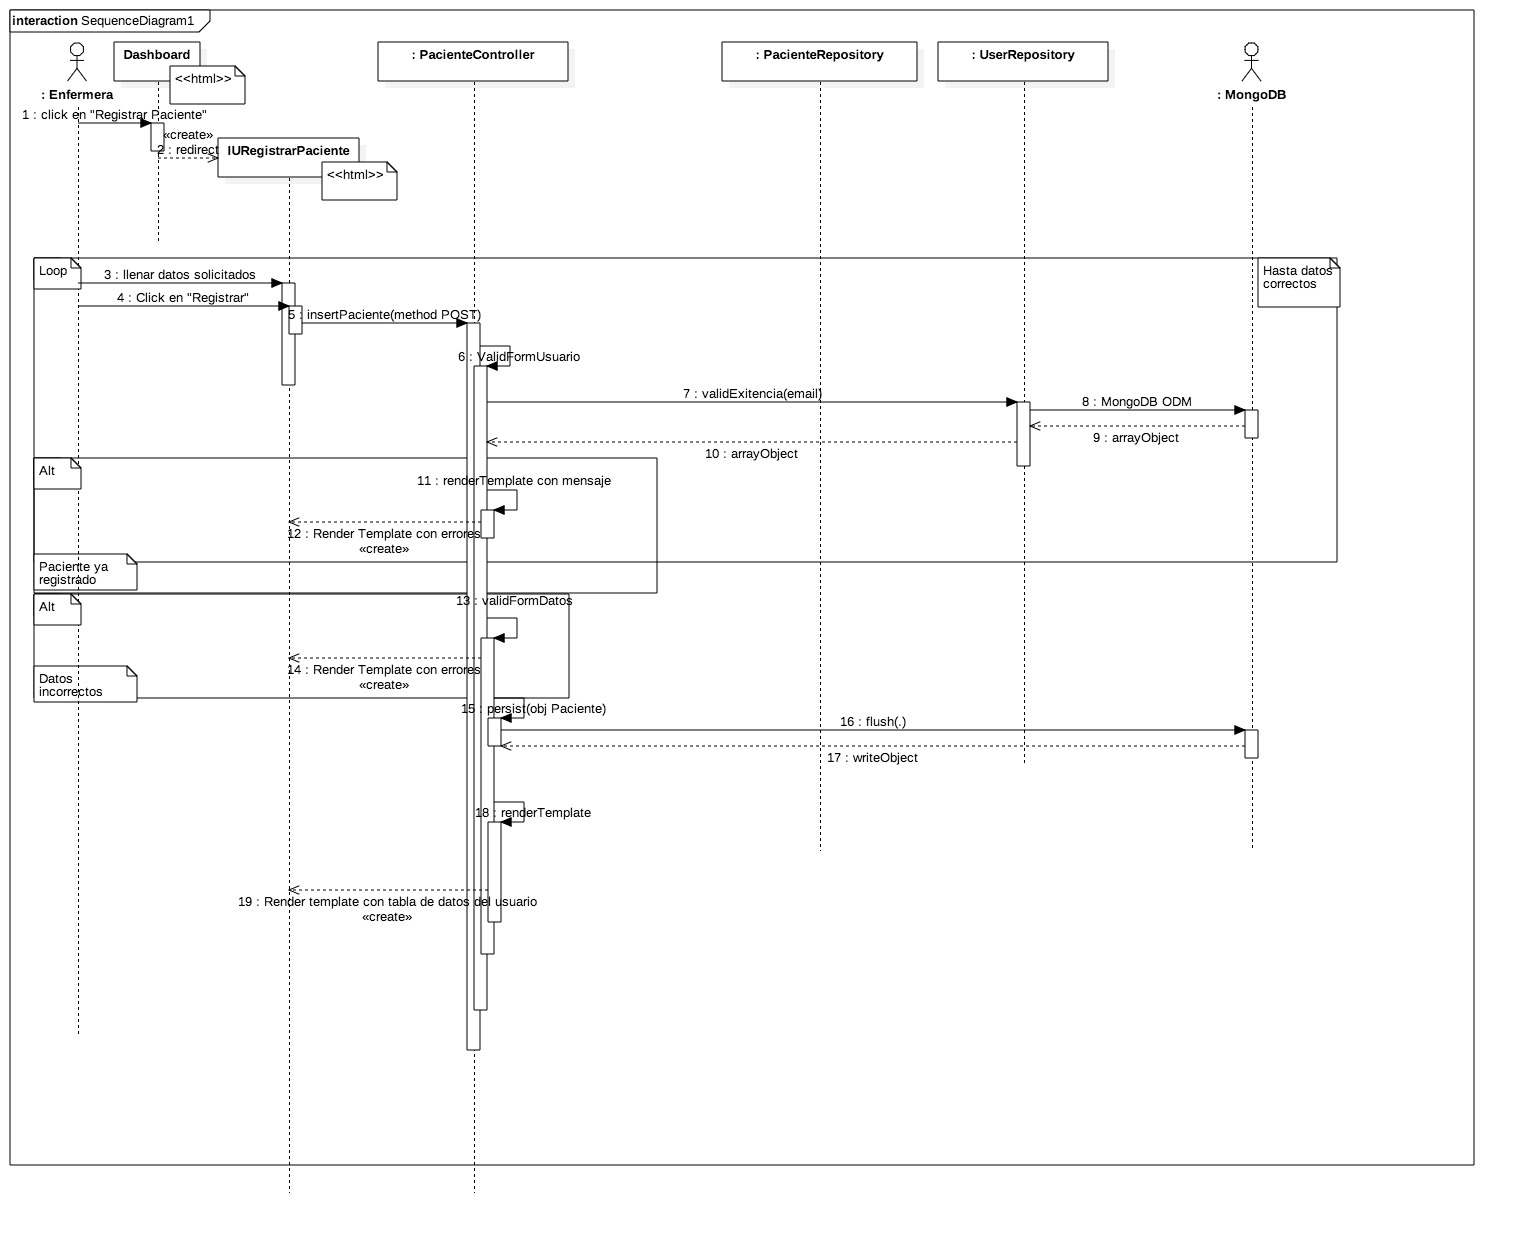
\includegraphics[width=1\textwidth]{uml/DiagramasSecuencia/RubenMurga/insertPaciente}
		\caption{Registrar Paciente}
	\end{figure}